\documentclass[tikz,border=5pt]{standalone}
\usepackage[utf8]{inputenc}
\usepackage[T1]{fontenc}
\usepackage{graphicx}

\begin{document}
	\begin{tikzpicture}[
		box/.style={draw, rectangle, minimum width=2cm, minimum height=1cm, align=center},
		title/.style={font=\large\bfseries}
		]
		
		% Título
		\node[title] at (0, 3) {Programa Genes};
		
		% Imagem central
		\node at (0, 4) {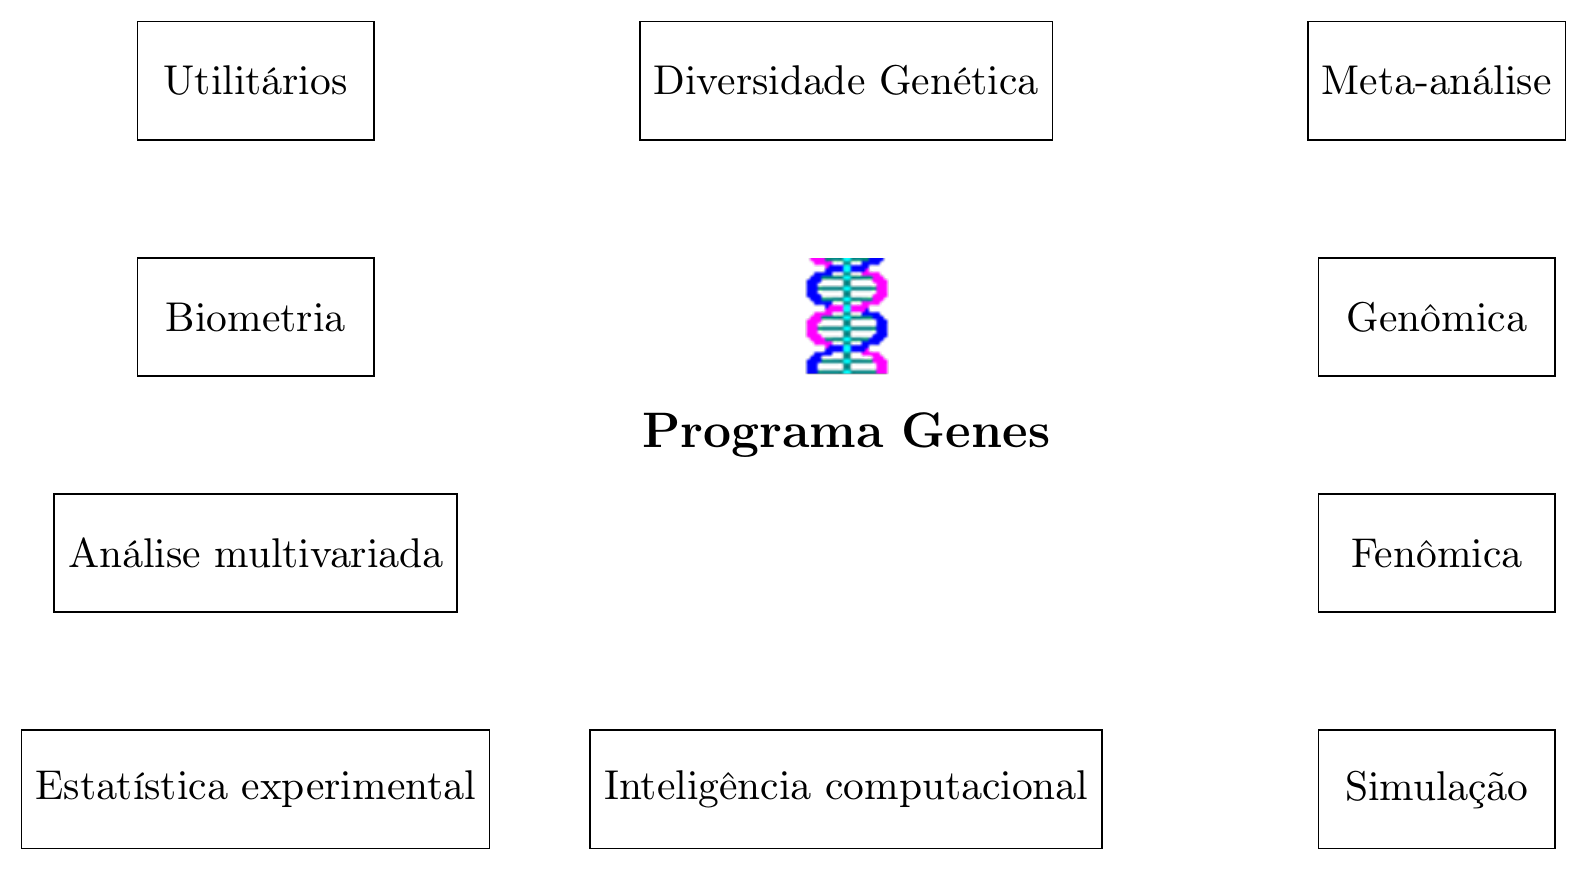
\includegraphics[width=1cm]{genes.png}};
		
		% Caixas do lado ESQUERDO (4 caixas)
		\node[box] at (-5, 6) {Utilitários};
		\node[box] at (-5, 4) {Biometria};
		\node[box] at (-5, 2) {Análise multivariada};
		\node[box] at (-5, 0) {Estatística experimental};
		
		% Caixas do lado DIREITO (4 caixas)
		\node[box] at (5, 6) {Meta-análise};
		\node[box] at (5, 4) {Genômica};
		\node[box] at (5, 2) {Fenômica};
		\node[box] at (5, 0) {Simulação};
		
		% Caixa ACIMA
		\node[box] at (0, 6) {Diversidade Genética};
		
		% Caixa ABAIXO
		\node[box] at (0, 0) {Inteligência computacional};
		
	\end{tikzpicture}
\end{document}